\chapter{Resultados Parciais e Discussões}\label{resultados}

\section{Simulação da Temperatura}

\subsection{Simulação do perfil térmico em 1D}

A equação \ref{eq:simplificada} foi resolvida analiticamente com os parâmetros descritos em \ref{teste_alg} e a solução encontrada é dada pela equação \ref{eq:sol_1d}.

\begin{equation}\label{eq:sol_1d}
T(x) = 120+(100 \cdot e - 60) \cdot x-(100 \cdot e^x)
\end{equation}

Este resultado é mostrado na figura \ref{fig:dif_fin_1d}, onde ele é comparado com vários métodos para resolução das equações de diferenças finitas. Nele, o espaço (de 0 a 1m) foi discretizado em 100 pontos e os métodos iterativos utilizaram 2000 iterações. 

\begin{figure}[H]
\centering
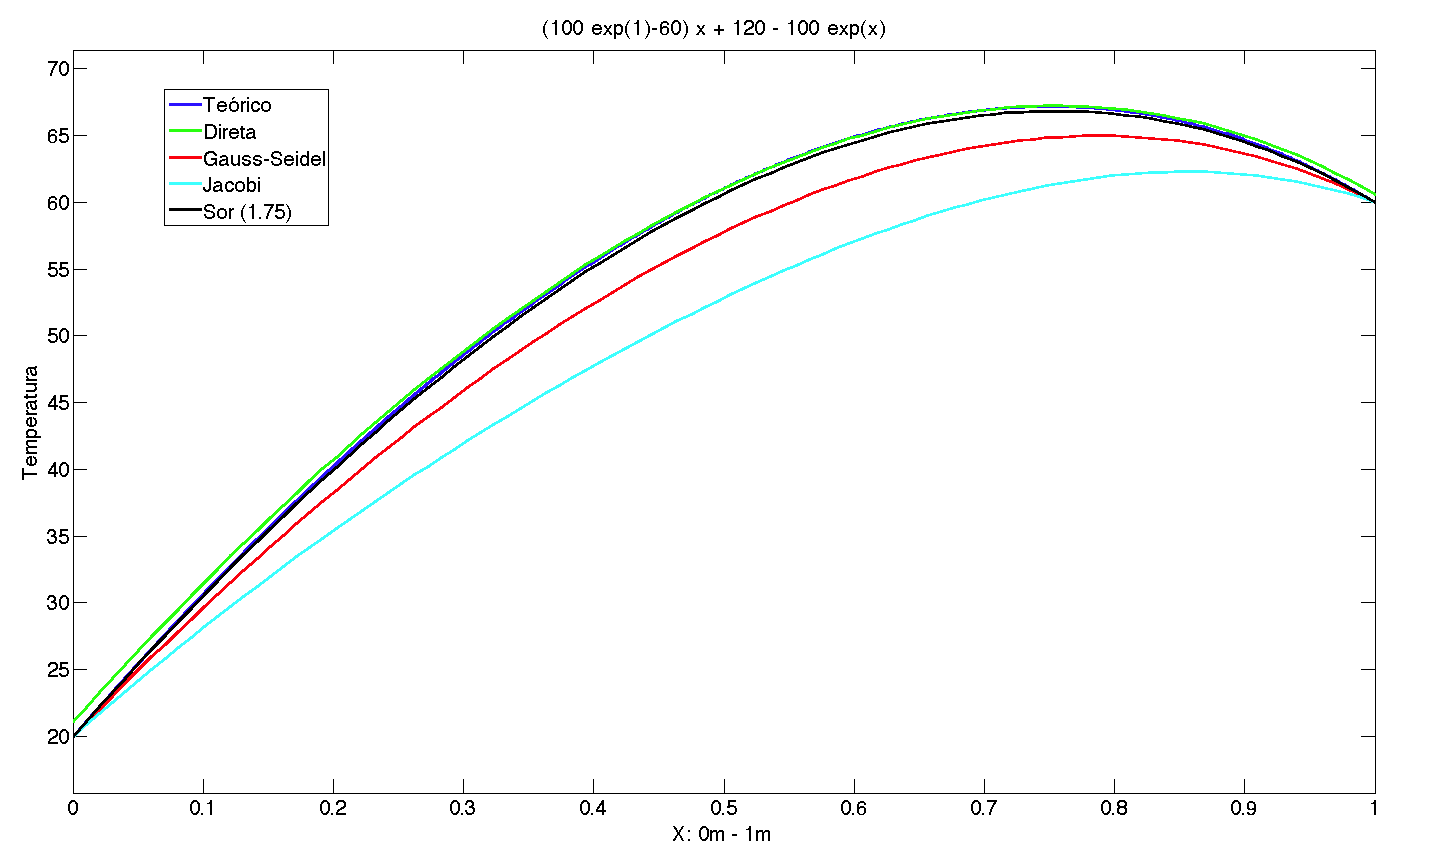
\includegraphics[width=\textwidth]{Figuras/dif_fin_1d}
\caption{Vários Algoritmos de Diferenças finitas em 1d}
\label{fig:dif_fin_1d}
\end{figure}
Como pode ser observado na figura \ref{fig:dif_fin_1d}, os métodos direto e SOR tiveram o melhor resultado, se aproximando da solução analítica. Com mais iterações todos os métodos iterativo convergem porém o método de Jacobi foi é o que necessita de mais iterações, seguido pelo método de Gauss-Seidel e o SOR foi o método iterativo que apresentou melhor resultado. 

Também foi testado o tempo necessário para a convergência dos vários métodos. Como os métodos iterativos convergem assintóticamente, foi estabelecido um erro limite para testar a quantidade de iterações para convergência. Este erro foi definido como a diferença entre a solução direta e o método direto, para que este também pudesse entrar na comparação de forma justa. 

Os valores para o resultado estão apresentados na tabela \ref{tab:tempo_metodos}. 

\begin{table}[htbp]
    \caption{Tempo de execução e número de iterações necessárias para se resolver o problema da difusão térmica 1D, comparado com solução analítica (erro < 0.001) }
    \label{tab:tempo_metodos}
    \vspace{1em}
    \centering
    \begin{tabular}{l r r r r}
        \toprule
        Método  	        & Tempo (s)             & Tempo Normalizado & Iterações     	\\
        \midrule
        Direto   	        & $6,44 \cdot 10^{-4}$  & 1,058	            & - 		        \\
        Jacobi	            & $1,85 \cdot 10^{-1}$  & 302,1             & 12475             \\
        Gauss-Seidel   	    & $3,82 \cdot 10^{-2}$	& 62,73		        &  6240		        \\
        SOR            	    & $6,09 \cdot 10^{-4}$	& 1,000		        &    76		        \\
        \bottomrule
    \end{tabular}
\end{table}

Com este resultado, observamos que o método SOR e o método direto foram os mais eficientes em resolver o problema. O método SOR foi o escolhido como o melhor candidato a ser utilizado na simulação devido a escalabilidade para sistemas 2D e 3D, onde resolver a matriz dos coeficientes (equação \ref{eq:matricial}) demanda um tempo que cresce exponencialmente em relação ao tamanho da matriz.  

\subsection{Parâmetro $w$ no método SOR}

Para determinar o melhor parâmetro $w$ do método SOR, o algoritmo foi executado até que se atingisse um erro fixo entre a solução analítica (anexo \ref{alg:sor}. Então, o algoritmo foi executado consecutivamente para valores de $w$ entre 1 e 1,99, com passo de 0,05. Uma contagem do número de iterações necessárias para a convergência foi feita em função de w e o resultado é apresentado na figura \ref{fig:parametro_sor}. O melhor valor de $w$, para o qual a convergência é mais rápida, foi o valor de 1,965.

\begin{figure}[H]
\centering
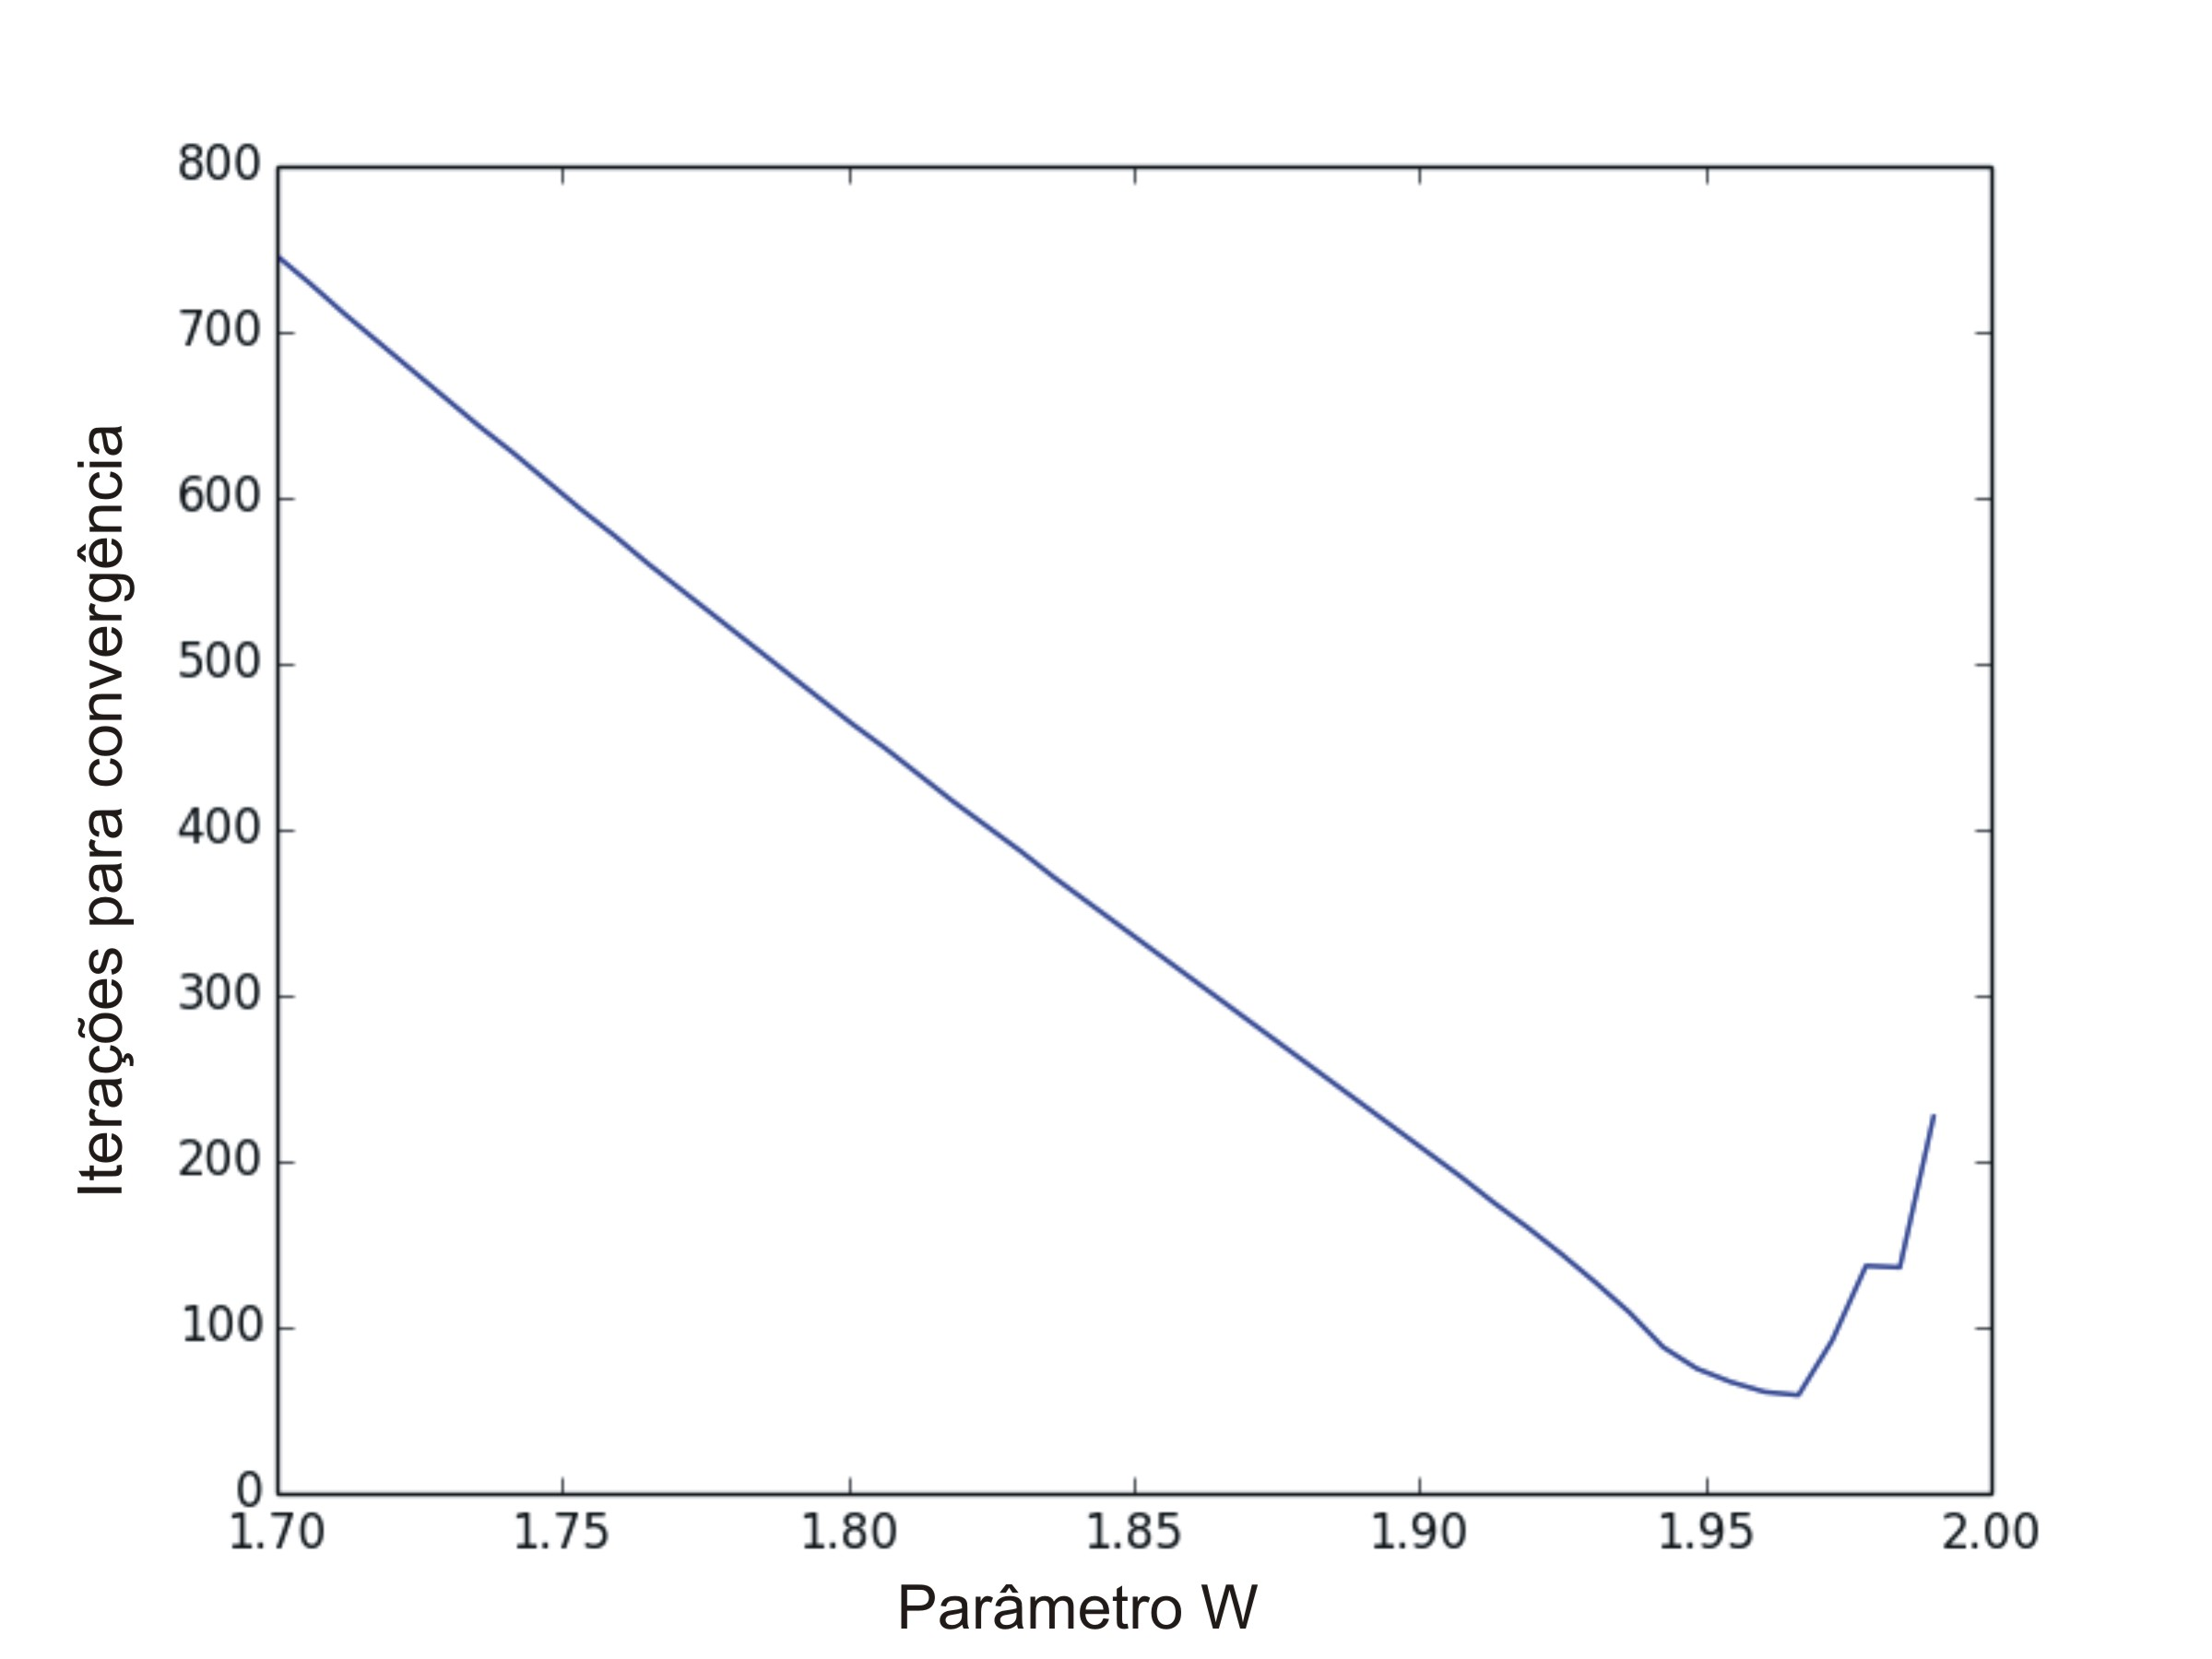
\includegraphics[width=\textwidth]{Figuras/parametro_sor}
\caption{Algoritmo SOR: Número de iterações em função de $w$}
\label{fig:parametro_sor}
\end{figure}

\subsection{Eficiência computacional do algoritmo em várias linguagens}

Para comparar a eficiência computacional do mesmo algoritmo em várias linguagens foi escolhido o método SOR e as linguagens escolhidas foram C/C++, Fortran, Python, Matlab e Octave. Os códigos respectivos encontram-se no anexo \ref{alg:linguagens}, sendo que o mesmo código foi utilizado para o matlab e para o octave, já que a sintaxe é a mesma. Os resultados estão apresentados na tabela \ref{tab:tempo_sor}

\begin{table}[htbp]
    \caption{Tempo de execução do Código de Diferenças Finitas 1D - SOR em várias linguagens}
    \label{tab:tempo_sor}
    \vspace{1em}
    \centering
    \begin{tabular}{l r r r r}
        \toprule
        Linguagem	        & Tempo (s)     & Tempo Normalizado & Desvio Padrão	    \\
        \midrule
        C/C++   	        & 0,007168		& 1,000	            & $9,707 \cdot 10^{-6}$	\\
        Fortran	            & 0,007184      & 1,0023            & $9,797 \cdot 10^{-6}$ \\
        Python/Numpy   	    & 0,070621		& 9,8528		    & $5,997 \cdot 10^{-4}$	\\
        Python-loop   	    & 1,506437		& 210,17		    & $6,73 \cdot 10^{-2}$		    \\
        Matlab-loop   	    & 0,064592		& 9,0116		    & $8,114 \cdot 10^{-4}$	\\
        Matlab-vetorizado   & 0,044488	    & 6,2067		    & $3,197 \cdot 10^{-3}$  \\
        Octave-loop   	    & 7,710252	    & 1075,7		    & $8,3 \cdot 10^{-2}$		    \\
        Octave-vetorizado   & 0,173330		& 24,182		    & $9,48 \cdot 10e^{-4}$ \\
        \bottomrule
    \end{tabular}
\end{table}

As linguagens C/C++ e Fortran foram as que obtiveram melhores resultados, como já era esperado, pois se tratam de linguagens compiladas altamente otimizadas para performance. Nas linguagens interpretadas, notamos uma diferença significativa entre os algoritmos vetorizados e não vetorizados, uma vez a vetorização, tanto no matlab, quanto no octave e no numpy, utilizam rotinas em C (Matlab e Octave) ou Fortran (numpy).

Ambas as linguagens compiladas se mostraram satisfatórias para a execução da simulação, com tempo de execução muito abaixo da ordem de grandeza do tempo de resposta do forno. No entanto, testes em sistemas embarcados ainda devem ser feitos para se averiguar a queda de performance.

\subsection{Eficiência computacional do algoritmo em vários sistemas embarcados}

Nesta etapa, será comparado o mesmo algoritmo em uma linguagem escolhida em vários sistemas embarcados para que se possa escolher o sistema mais adequado. Caso o tempo de simulação esteja muito abaixo do tempo necessário pelo controle PID, será escolhido o hardware que possua mais benefícios em termos de compatibilidade, usabilidade e preço.

\section{Controle}

\subsection{Reconhecimento de Imagem}

Os testes iniciais mostram que o algoritmo utilizado foi capaz de captar os objetos de acordo com o formato e a cor, não gerando falsos positivos e errando apenas quando o alimento não estava no padrão que deveria figura \ref{fig:opencv}.  

Para o filtro de cores, o melhor resultado foi obtido realizando uma transformada do espectro RGB para HSV, garantindo que seja buscada apenas um range específico de cor e que o brilho e iluminação não interferissem no resultado.  

\begin{figure}[htbp]
    \centering
    \subfloat[Entrada]{\label{fig:Entrada}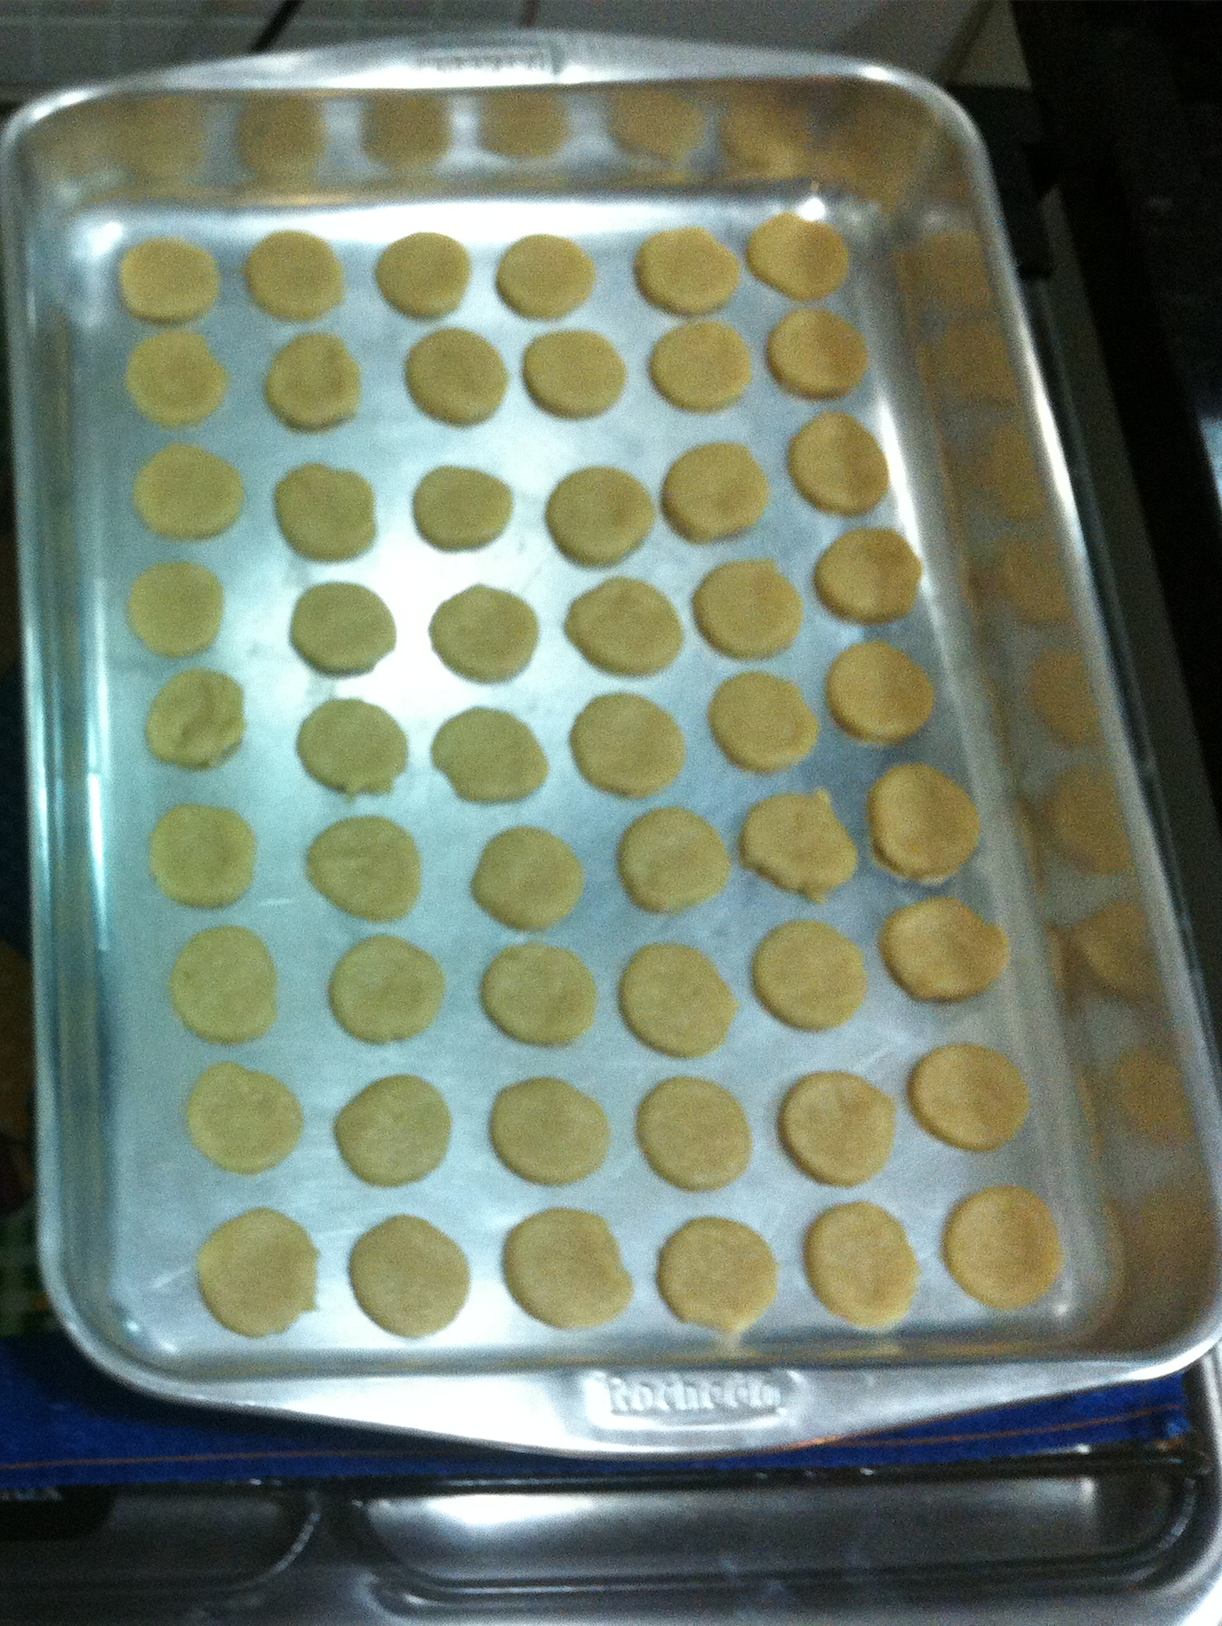
\includegraphics[width=200pt]{Figuras/imagens_biscoito/antes}}\vspace{11pt}
    \subfloat[Filtro Limiar Adaptativo]{\label{fig:filtro_limiar}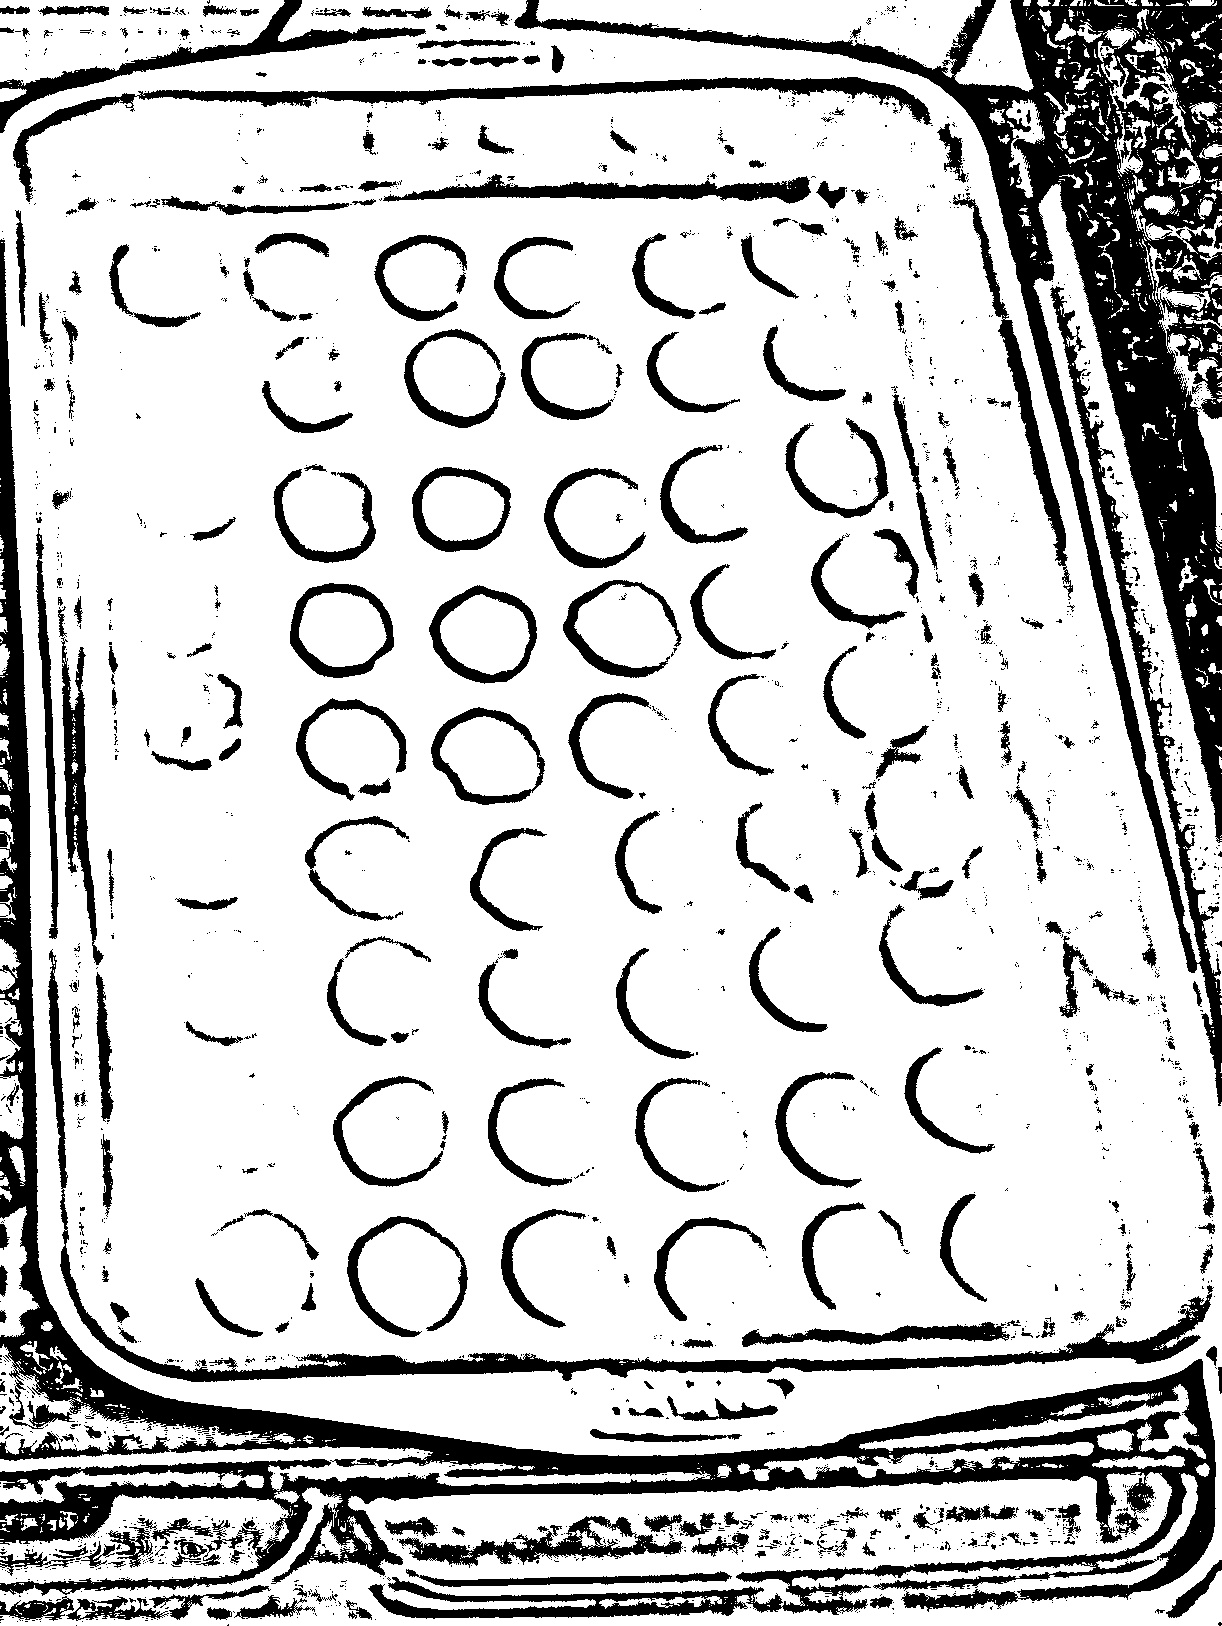
\includegraphics[width=200pt]{Figuras/imagens_biscoito/biscoito_limiar}}\\
    \vspace{-18pt}
    \subfloat[Filtro HSV]{\label{fig:filtro_hsv}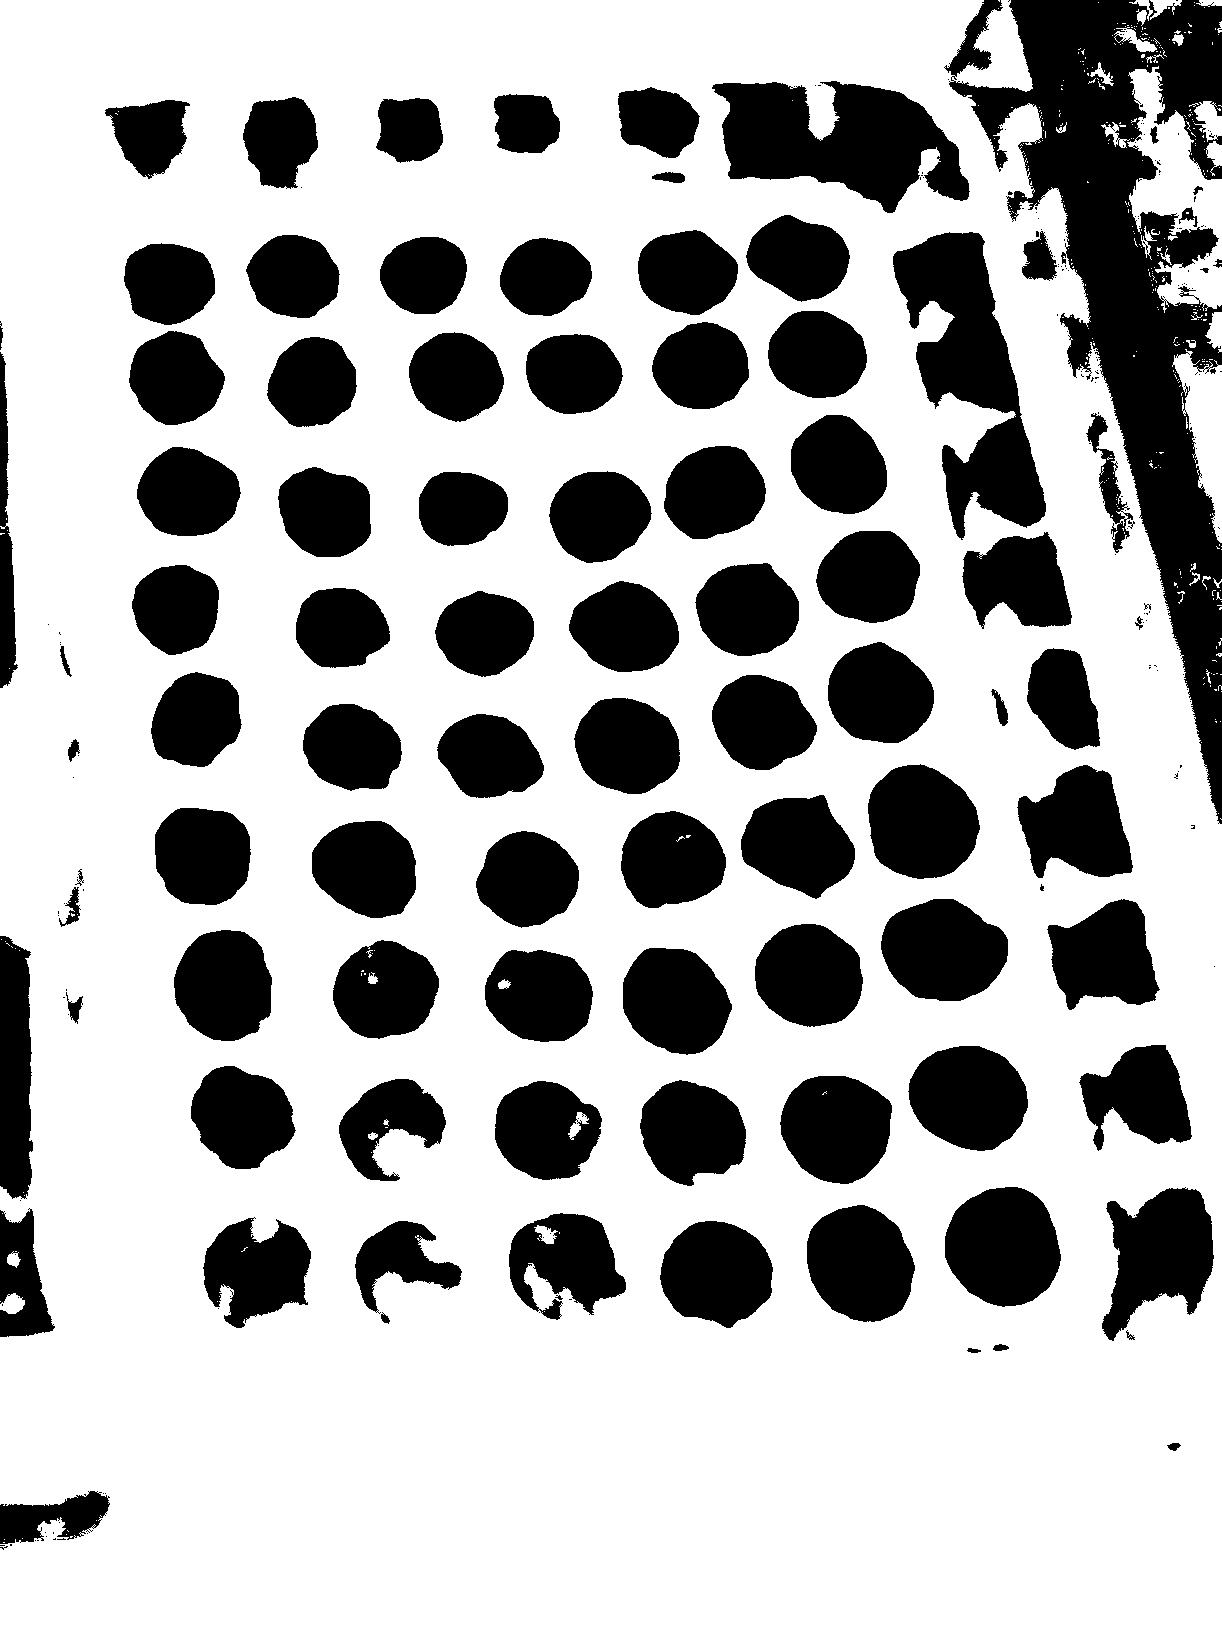
\includegraphics[width=200pt]{Figuras/imagens_biscoito/biscoito_filtro_cor}}\vspace{11pt}
    \subfloat[Objetos redondos reconhecidos]{\label{fig:redondo}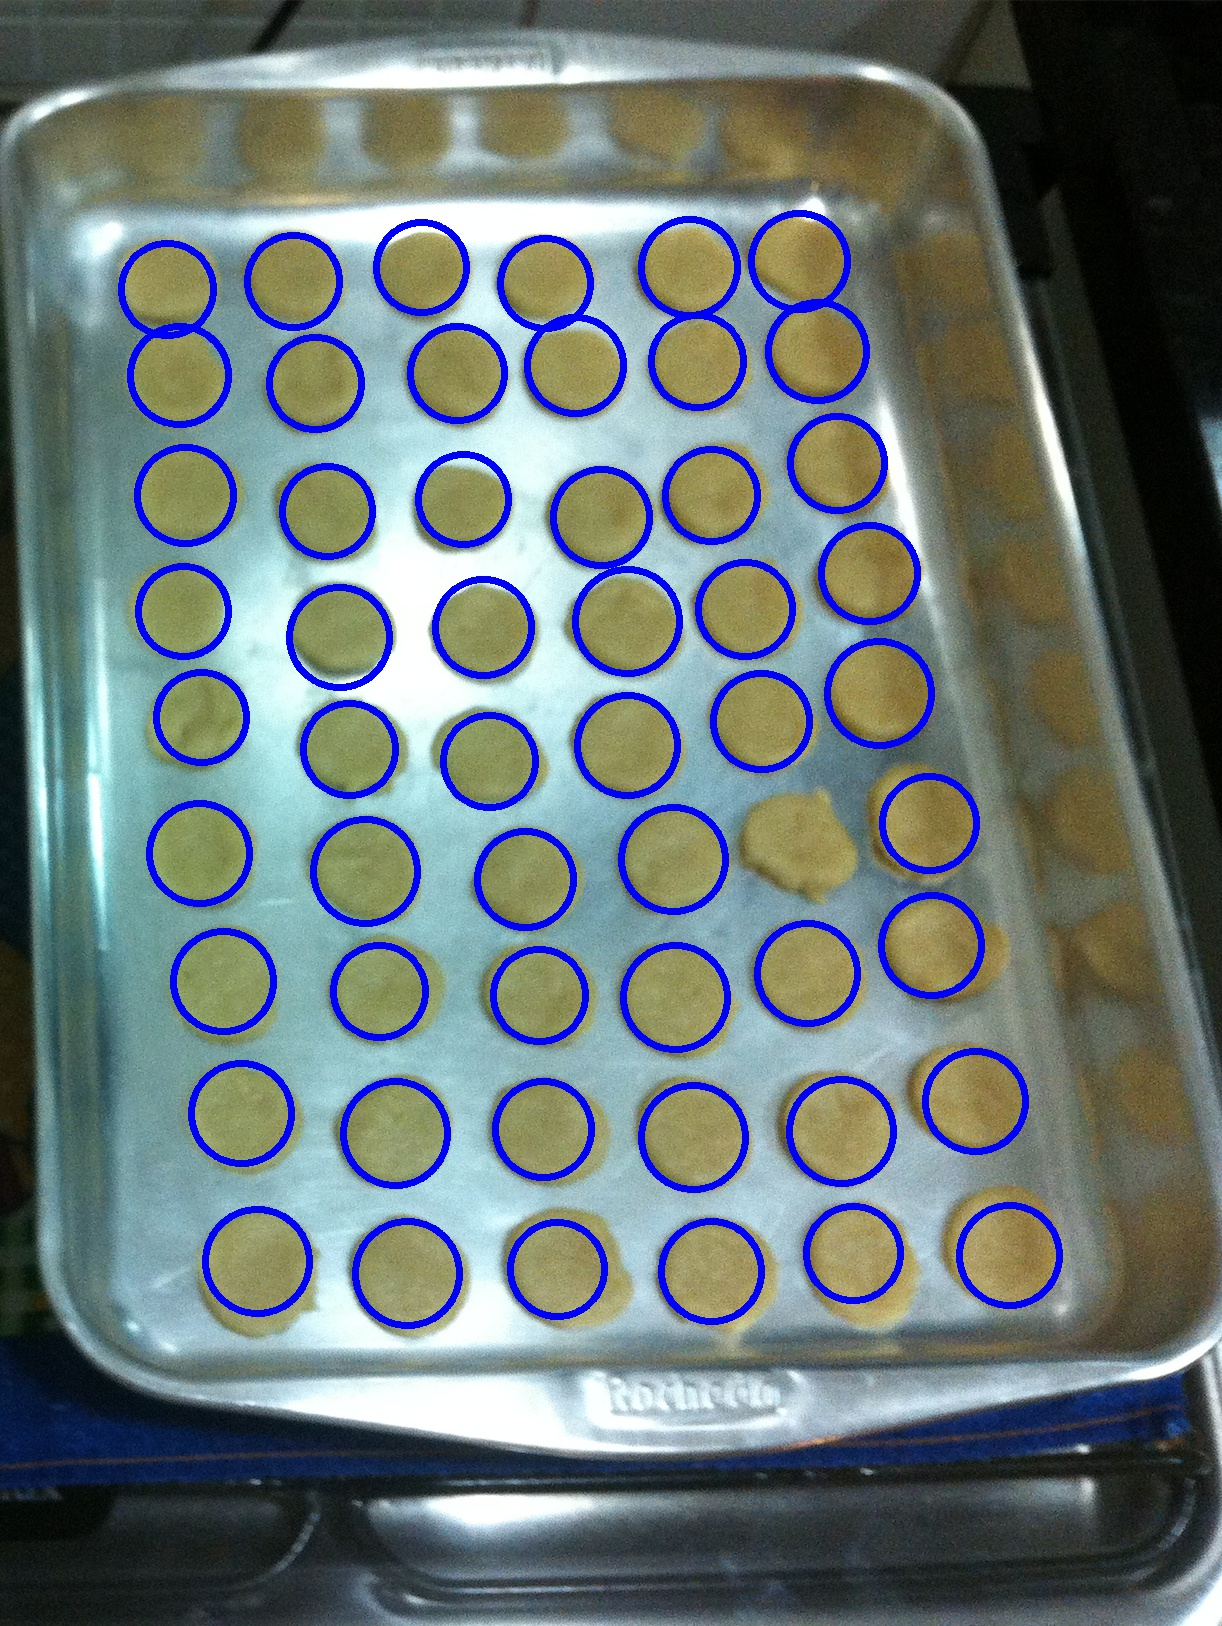
\includegraphics[width=200pt]{Figuras/imagens_biscoito/biscoito_reconhecido}}
    \caption{Processamento da imagem, iniciando com a imagem pura (a), aplicação de filtros limiar adaptativo (b), filtro HSV (c) e por último o reconhecimento dos objetos redondos na imagem tratada (d)}
    \label{fig:opencv}
\end{figure}

Após a aplicação do filtro de cores, foi aplicado um limiar binário, para preparar a imagem para o reconhecimento de formatos (no caso do teste, de objetos redondos). O limiar utilizado foi o adaptativo com filtro gaussiano (anexo \ref{alg:camera}, de modo que não dependesse de um limiar fixo, que pode alterar a detecção caso as condições de claridade sejam alterados.

Os resultados foram satisfatórios na detecção de biscoitos redondos e futuros testes utilizando as informações da área e quantidade de biscoitos reconhecidos será feita para estivar a massa total que entrará no forno. Estes dados poderão ser inseridos no algoritmo de controle caso a massa seja um parâmetro que possa alterar o perfil de temperatura.

Um fator importante da coleta de imagem é o controle de qualidade, possibilitando que o sistema possa ser alterado para controlar a qualidade do produto produzido. 

\subsection{Software de Controle - Interface gráfica}

Na figura \ref{fig:gui_control} vemos o resultado da interface gráfica produzida. Ela permite o controle automático e manual do forno, mas a integração de todos os códigos de simulação ao controle automático ainda não foram realizados devido a necessidade de testes do controle PID. 

Testes qualitativos mostraram indicam que a interface funcionou corretamente mas testes futuros ainda deverão ser feitos. Uma outra possibilidade que será analisada é a utilização de uma interface gráfica via web, diminuindo a necessidade de uso da memória para processamento gráfico, uma vez que isto será feito do lado do “cliente” e não do servidor. 

\begin{figure}[H]
\centering
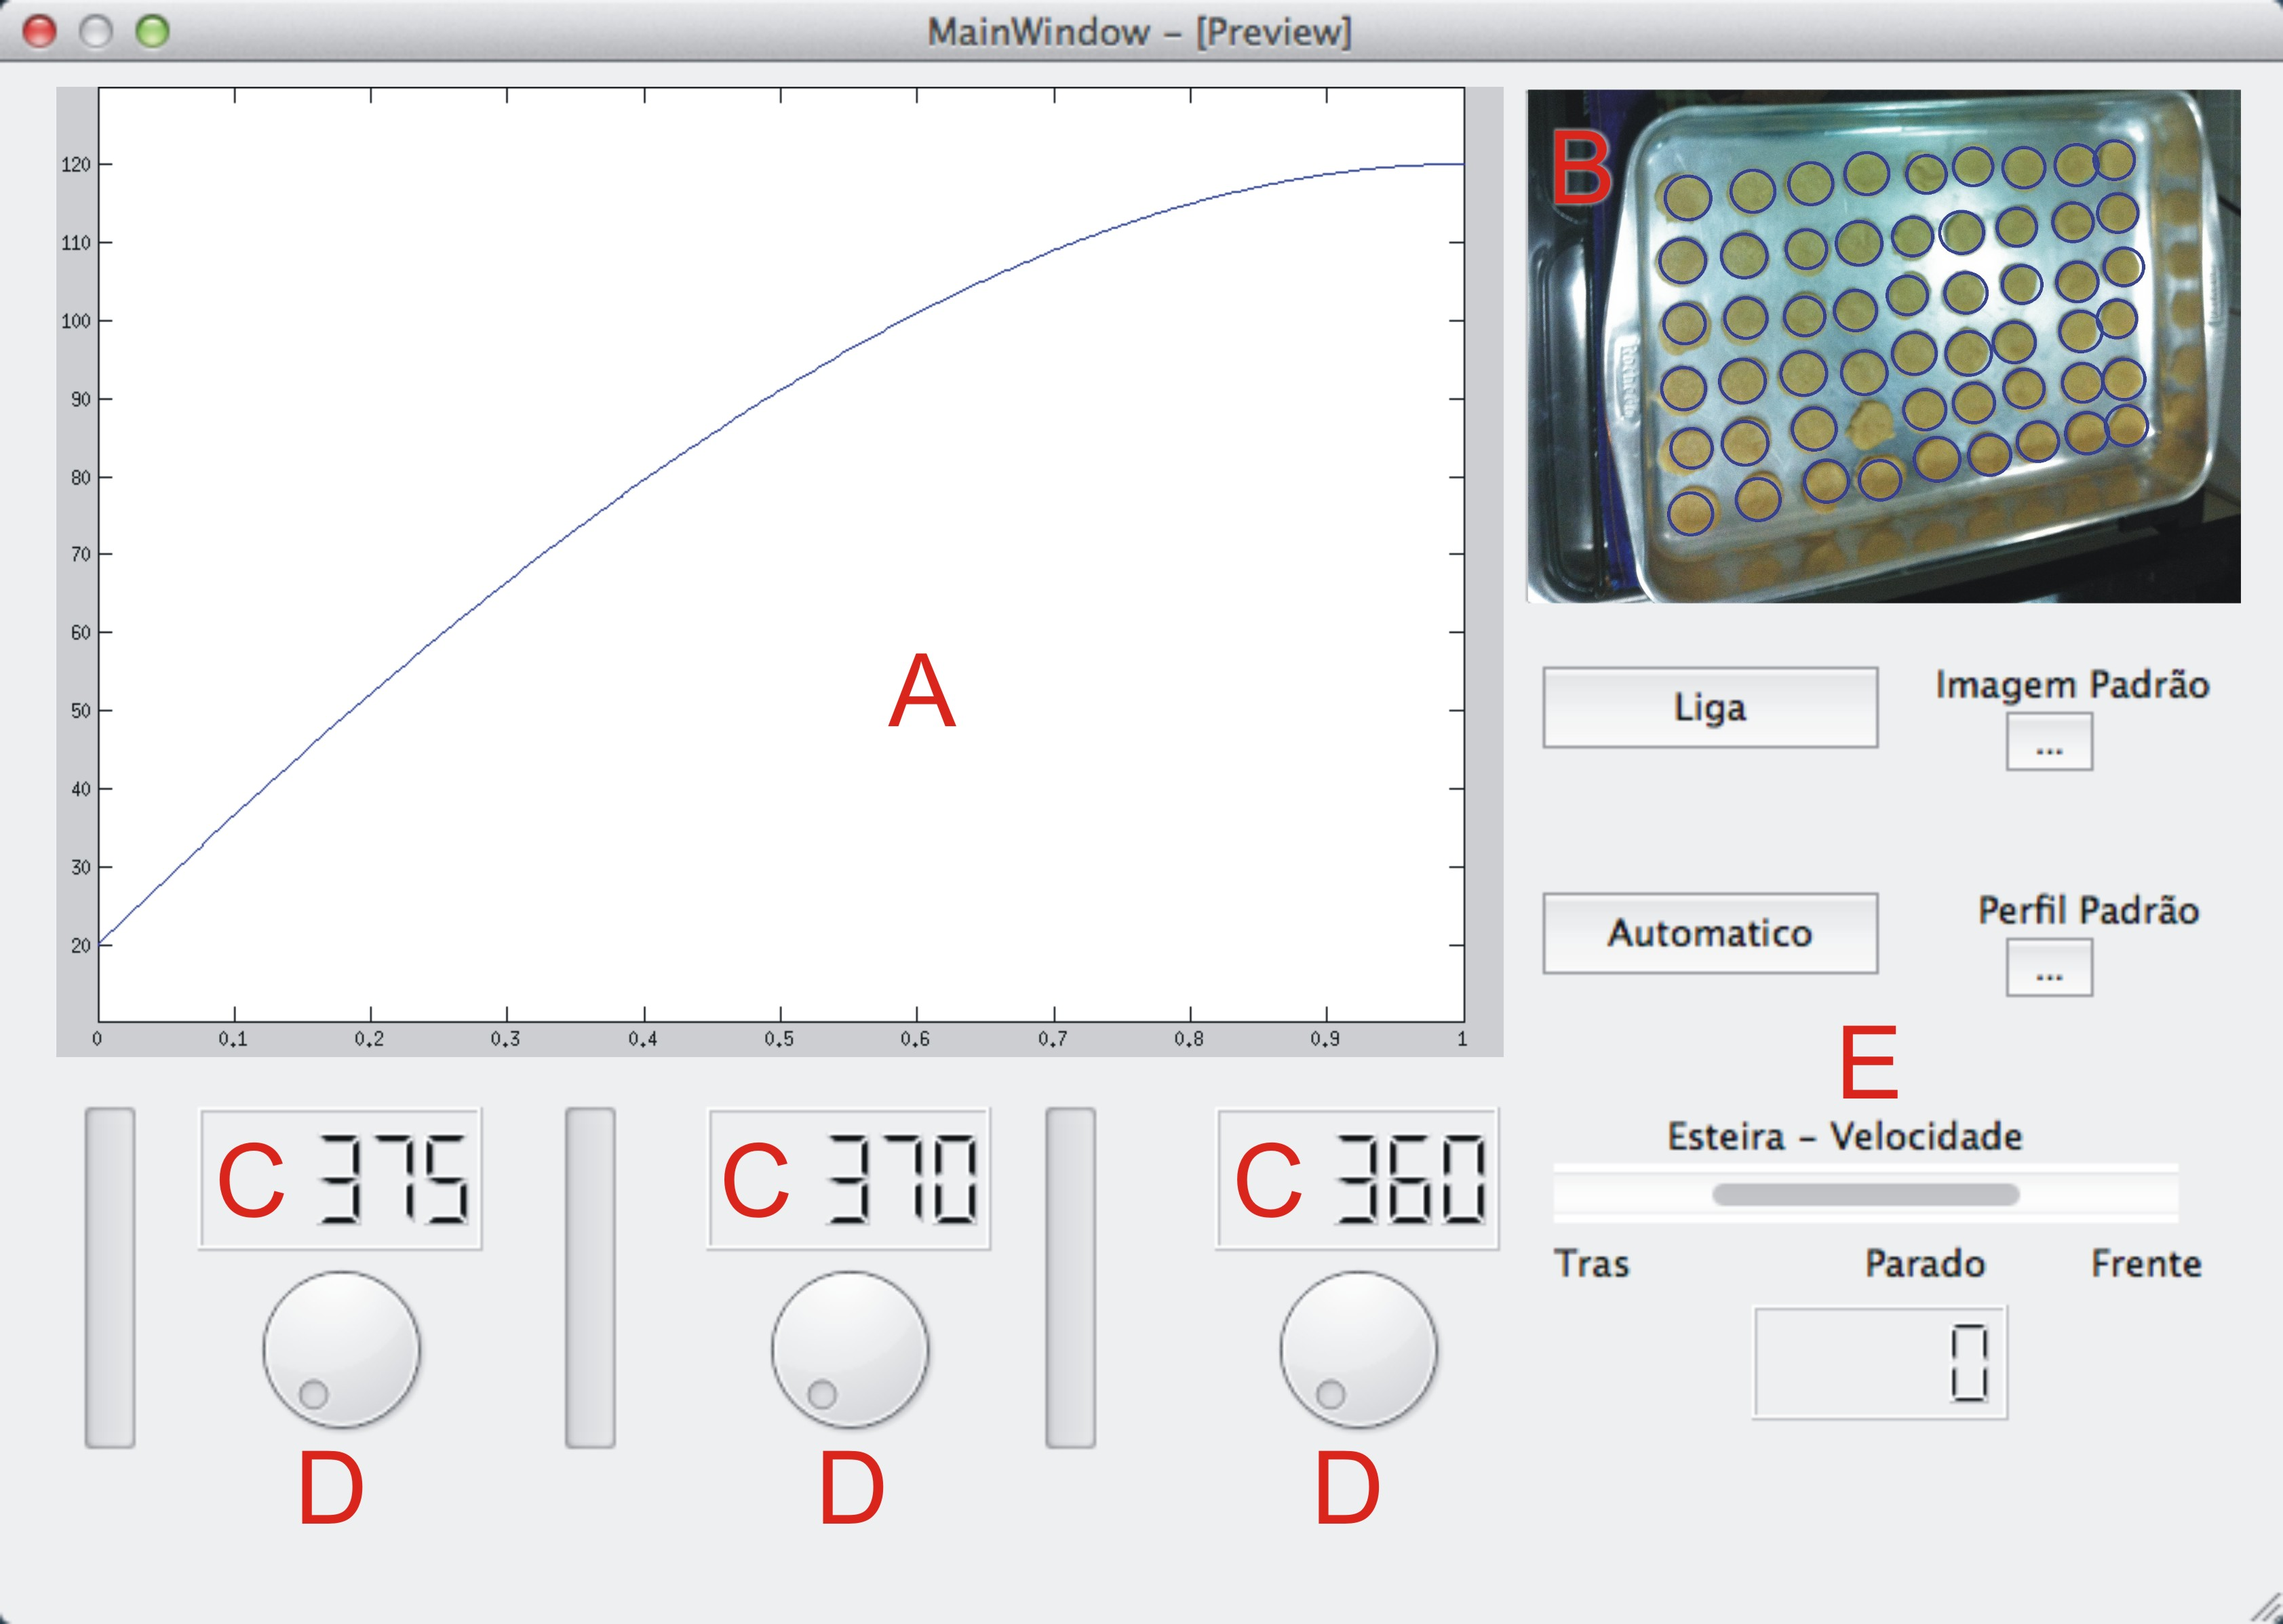
\includegraphics[width=\textwidth]{Figuras/gui_control2}
\caption{Software de controle. A: Resultado da simulação térmica ao longo do perfil do forno. B: Imagem da Câmera na entrada do forno com reconhecimento de padrão. C: Leitura do sensor de temperatura nas três zonas térmicas. D: Controle manual a potência nas três zonas térmicas. E: Controle manual da velocidade da esteira.}
\label{fig:gui_control}
\end{figure}






















